\documentclass[border=4pt,12pt]{standalone}
% House style for redrawn exam diagrams (diagram-v4: 0.4pt lines, filled -latex arrows, fine dashes; stipple and hatching drawn as real dots/lines (no PDF/SVG patterns, so they render in every browser and at any scale); transparent background). Every figure \input's this.
\usepackage{amsmath,amssymb}
\usepackage{txfonts}
\usepackage{pdfrender,xcolor}
% \halo{text}: label on shading. The shading stops just around each letter's outline (a thin knock-out that follows the
% glyphs, like the papers' typesetting), never a box. Owner: "I don't want a box around the text".
\newcommand{\halo}[1]{\leavevmode\rlap{\pdfrender{TextRenderingMode=2,LineWidth=2.2pt,LineJoinStyle=1,StrokeColor=white,FillColor=white}#1}#1}
\usepackage{tikz,pgfplots}
\pgfplotsset{compat=1.18}
\usetikzlibrary{arrows.meta,calc,angles,quotes,patterns,patterns.meta,intersections,positioning,decorations.markings,shapes.geometric}
% Stipple and hatching are drawn as actual dots / lines clipped to the region (path picture), NOT as pattern fills:
% SVG <pattern> fills vanish or blur when browsers scale the image, so the owner could not see the shading.
% Each dot is a 0.72pt square (keeps SVGs small; reads as a dot at print size). Dots sit on one global staggered grid, so neighbouring regions line up.
\makeatletter
\newdimen\ex@x \newdimen\ex@y \newdimen\ex@xa \newdimen\ex@ya \newdimen\ex@xb \newdimen\ex@yb \newcount\ex@row
\def\exam@stipplecolor{black!75}\def\exam@dotr{0.42pt}\def\exam@dotgap{2.5}
\def\ex@rowdots{\ifdim\ex@x<\ex@xb \pgfpathrectangle{\pgfqpoint{\dimexpr\ex@x-0.36pt\relax}{\dimexpr\ex@y-0.36pt\relax}}{\pgfqpoint{0.72pt}{0.72pt}}\advance\ex@x by \exam@dotgap pt\relax\expandafter\ex@rowdots\fi}
\def\exam@stipple{%
  \pgftransformreset% dots are sized in real points even inside scaled pictures
  \pgfpointanchor{path picture bounding box}{south west}\ex@xa=\pgf@x \ex@ya=\pgf@y
  \pgfpointanchor{path picture bounding box}{north east}\ex@xb=\pgf@x \ex@yb=\pgf@y
  \pgfsetfillcolor{\exam@stipplecolor}\pgfmathsetmacro\ex@h{\exam@dotgap/2}%
  \pgfmathtruncatemacro\ex@r{floor(\ex@ya/\ex@h)-1}\ex@row=\ex@r\relax
  \ex@y=\ex@r\dimexpr\ex@h pt\relax
  \loop\ifdim\ex@y<\ex@yb
    \pgfmathtruncatemacro\ex@c{floor(\ex@xa/\exam@dotgap)-1}\ex@x=\ex@c\dimexpr\exam@dotgap pt\relax
    \ifodd\ex@row \advance\ex@x by \ex@h pt\fi
    \ex@rowdots
    \advance\ex@y by \ex@h pt \advance\ex@row by 1
    \ifnum\numexpr\ex@row-(\ex@row/4)*4\relax=0 \pgfusepath{fill}\fi% flush every 4 rows: bounded TeX memory, few clip copies in the SVG
  \repeat\pgfusepath{fill}}
\newdimen\ex@d
\def\exam@hatch#1{% #1 = 1 for /, -1 for \ ; lines 45 degrees, 3pt apart
  \pgftransformreset
  \pgfpointanchor{path picture bounding box}{south west}\ex@xa=\pgf@x \ex@ya=\pgf@y
  \pgfpointanchor{path picture bounding box}{north east}\ex@xb=\pgf@x \ex@yb=\pgf@y
  \ex@d=\dimexpr\ex@yb-\ex@ya\relax \ex@x=\dimexpr\ex@xa-\ex@d\relax
  \loop\ifdim\ex@x<\ex@xb
    \ifnum#1>0 \pgfpathmoveto{\pgfqpoint{\ex@x}{\ex@ya}}\pgfpathlineto{\pgfqpoint{\dimexpr\ex@x+\ex@d\relax}{\ex@yb}}%
    \else \pgfpathmoveto{\pgfqpoint{\ex@x}{\ex@yb}}\pgfpathlineto{\pgfqpoint{\dimexpr\ex@x+\ex@d\relax}{\ex@ya}}\fi
    \advance\ex@x by 4.24pt
  \repeat
  \pgfsetlinewidth{0.4pt}\pgfsetstrokecolor{black}\pgfusepath{stroke}}
\def\examstipple{\exam@stipple}\def\examhatch{\exam@hatch}\def\examsetstipplecolor#1{\def\exam@stipplecolor{#1}}\def\examsetdotgap#1{\def\exam@dotgap{#1}}
\makeatother
% (legacy pattern kept for old files)
% staggered stipple like the NESA papers' dotted shading
\pgfdeclarepatternformonly{exam stipple}{\pgfpointorigin}{\pgfqpoint{2.2pt}{2.2pt}}{\pgfqpoint{2.2pt}{2.2pt}}{%
  \pgfpathcircle{\pgfqpoint{0.55pt}{0.55pt}}{0.42pt}\pgfpathcircle{\pgfqpoint{1.65pt}{1.65pt}}{0.42pt}\pgfusepath{fill}}
\tikzset{
  every picture/.style={line width=0.6pt, >={Latex[length=2mm,width=1.3mm]}},
  curve/.style={line width=0.6pt},
  open arrow/.style={-{Latex[length=2mm,width=1.3mm]}},  % owner: filled -latex heads everywhere, no open chevrons
  aux/.style={dash pattern=on 2pt off 1.5pt, line width=0.6pt},
  shade/.code={\def\exA{#1}\def\exB{none}\ifx\exA\exB\else\pgfkeysalso{fill=black!18}\fi},
  shade/.default=on,
  shade dots/.style={fill=none, path picture={\examstipple}},
  stipple color/.code={\examsetstipplecolor{#1}},
  stipple gap/.code={\examsetdotgap{#1}},
  shade dense dots/.style={fill=none, stipple gap=1.6, path picture={\examstipple}},
  shade hatch/.style={fill=none, path picture={\examhatch{1}}},
  shade hatch reverse/.style={fill=none, path picture={\examhatch{-1}}},
  shade solid/.style={fill=black},
  pt/.style={circle, fill, inner sep=1.1pt},
  open pt/.style={circle, draw, fill=white, inner sep=1.1pt},
}
\pgfplotsset{
  exam axes/.style={axis lines=middle, axis line style={->}, xlabel={$x$}, ylabel={$y$},
    xlabel style={anchor=west}, ylabel style={anchor=south}, tick label style={font=\small},
    every axis plot/.append style={line width=0.6pt, black}, samples=200, clip=false,
    enlargelimits=false, axis on top},
}

\begin{document}
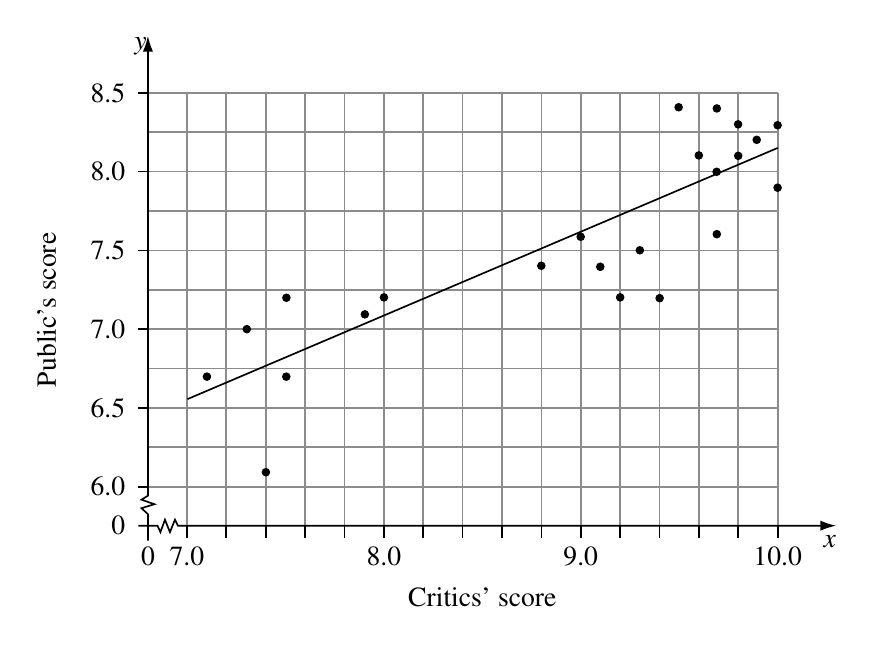
\begin{tikzpicture}[x=0.0127cm,y=-0.0127cm]
  \draw[black!45] (206.9,69) -- (206.9,502);
  \draw[black!45] (246.3,69) -- (246.3,502);
  \draw[black!45] (285.7,69) -- (285.7,502);
  \draw[black!45] (325.1,69) -- (325.1,502);
  \draw[black!45] (364.5,69) -- (364.5,502);
  \draw[black!45] (403.9,69) -- (403.9,502);
  \draw[black!45] (443.3,69) -- (443.3,502);
  \draw[black!45] (482.7,69) -- (482.7,502);
  \draw[black!45] (522.1,69) -- (522.1,502);
  \draw[black!45] (561.5,69) -- (561.5,502);
  \draw[black!45] (600.9,69) -- (600.9,502);
  \draw[black!45] (640.3,69) -- (640.3,502);
  \draw[black!45] (679.7,69) -- (679.7,502);
  \draw[black!45] (719.1,69) -- (719.1,502);
  \draw[black!45] (758.5,69) -- (758.5,502);
  \draw[black!45] (167.5,69) -- (167.5,502);
  \draw[black!45] (128.5,463.0) -- (758.5,463.0);
  \draw[black!45] (128.5,423.6) -- (758.5,423.6);
  \draw[black!45] (128.5,384.2) -- (758.5,384.2);
  \draw[black!45] (128.5,344.8) -- (758.5,344.8);
  \draw[black!45] (128.5,305.4) -- (758.5,305.4);
  \draw[black!45] (128.5,266.0) -- (758.5,266.0);
  \draw[black!45] (128.5,226.6) -- (758.5,226.6);
  \draw[black!45] (128.5,187.2) -- (758.5,187.2);
  \draw[black!45] (128.5,147.8) -- (758.5,147.8);
  \draw[black!45] (128.5,108.4) -- (758.5,108.4);
  \draw[black!45] (128.5,69.0) -- (758.5,69.0);
  \draw (167.5,502) -- (167.5,514);
  \draw (206.9,502) -- (206.9,514);
  \draw (246.3,502) -- (246.3,514);
  \draw (285.7,502) -- (285.7,514);
  \draw (325.1,502) -- (325.1,514);
  \draw (364.5,502) -- (364.5,514);
  \draw (403.9,502) -- (403.9,514);
  \draw (443.3,502) -- (443.3,514);
  \draw (482.7,502) -- (482.7,514);
  \draw (522.1,502) -- (522.1,514);
  \draw (561.5,502) -- (561.5,514);
  \draw (600.9,502) -- (600.9,514);
  \draw (640.3,502) -- (640.3,514);
  \draw (679.7,502) -- (679.7,514);
  \draw (719.1,502) -- (719.1,514);
  \draw (758.5,502) -- (758.5,514);
  \draw (119,463.0) -- (128.5,463.0);
  \node[left, inner sep=0pt] at (106.5,463.0) {6.0};
  \draw (119,384.2) -- (128.5,384.2);
  \node[left, inner sep=0pt] at (106.5,384.2) {6.5};
  \draw (119,305.4) -- (128.5,305.4);
  \node[left, inner sep=0pt] at (106.5,305.4) {7.0};
  \draw (119,226.6) -- (128.5,226.6);
  \node[left, inner sep=0pt] at (106.5,226.6) {7.5};
  \draw (119,147.8) -- (128.5,147.8);
  \node[left, inner sep=0pt] at (106.5,147.8) {8.0};
  \draw (119,69.0) -- (128.5,69.0);
  \node[left, inner sep=0pt] at (106.5,69.0) {8.5};
  \node at (167.5,533) {7.0};
  \node at (364.5,533) {8.0};
  \node at (561.5,533) {9.0};
  \node at (758.5,533) {10.0};
  % axes with breaks (zigzags) as printed
  \draw[->] (128.5,517) -- (128.5,502) -- (128.5,490.5) -- (122,484.5) -- (135,480.5) -- (122,476) -- (128.5,472) -- (128.5,12);
  \draw[->] (119,502) -- (138,502) -- (141,508.5) -- (145.5,496) -- (150.5,508.5) -- (155.5,496) -- (158.5,502) -- (817,502);
  \draw (168,375.4) -- (758.5,124.1);
  \fill (659.4,83.4) circle[radius=4.3];
  \fill (697.6,84.6) circle[radius=4.3];
  \fill (718.9,100.5) circle[radius=4.3];
  \fill (758.4,101.4) circle[radius=4.3];
  \fill (737.5,116.0) circle[radius=4.3];
  \fill (679.6,131.6) circle[radius=4.3];
  \fill (719.0,132.0) circle[radius=4.3];
  \fill (697.4,148.0) circle[radius=4.3];
  \fill (758.4,163.9) circle[radius=4.3];
  \fill (697.6,210.4) circle[radius=4.3];
  \fill (561.4,213.0) circle[radius=4.3];
  \fill (620.6,226.5) circle[radius=4.3];
  \fill (522.0,242.0) circle[radius=4.3];
  \fill (581.0,243.0) circle[radius=4.3];
  \fill (267.0,274.0) circle[radius=4.3];
  \fill (364.6,273.6) circle[radius=4.3];
  \fill (600.9,273.6) circle[radius=4.3];
  \fill (640.4,274.4) circle[radius=4.3];
  \fill (345.5,290.6) circle[radius=4.3];
  \fill (227.4,305.4) circle[radius=4.3];
  \fill (187.5,352.9) circle[radius=4.3];
  \fill (266.9,352.9) circle[radius=4.3];
  \fill (246.5,448.5) circle[radius=4.3];
  \node[left, inner sep=0pt] at (106.5,502) {0};
  \node at (128.5,533) {0};
  \node at (121,22) {$y$};
  \node at (810,518) {$x$};
  \node at (463,574) {Critics' score};
  \node[rotate=90] at (27,286) {Public's score};
\end{tikzpicture}
\end{document}
